\item {\bf Kernelizing the Perceptron}

Let there be a binary classification problem with $y \in \{0, 1\}$.  The
perceptron uses hypotheses of the form $h_\theta(x) = g(\theta^T x)$, where
$g(z) = \text{sign}(z) = 1$ if $z \ge 0$, $0$ otherwise.  In this problem we
will consider a stochastic gradient descent-like implementation of the
perceptron algorithm where each update to the parameters $\theta$ is made using
only one training example.  However, unlike stochastic gradient descent, the
perceptron algorithm will only make one pass through the entire training set.
The update rule for this version of the perceptron algorithm is given by
\begin{equation*}
  \theta^{(i+1)} :=
	  \theta^{(i)} + \alpha (y^{(i+1)} - h_{\theta^{(i)}}(x^{(i+1)})) x^{(i+1)}
\end{equation*}
where $\theta^{(i)}$ is the value of the parameters after the algorithm has
seen the first $i$ training examples. Prior to seeing any training examples,
$\theta^{(0)}$ is initialized to $\vec{0}$.

\begin{enumerate}
  \input{03-perceptron/01-description}

  \item \points{3b} Implement your approach by completing the
\texttt{initial\_state}, \texttt{predict}, and \texttt{update\_state} methods
of \texttt{src-perceptron/submission.py}.


We provide two kernels, a dot-product kernel and a
radial basis function (RBF) kernel. 

Run \texttt{src-perceptron/submission.py} to train
kernelized perceptrons on \texttt{src-perceptron/train.csv}. The code will then test
the perceptron on \texttt{src-perceptron/test.csv} and save the resulting
predictions in the \texttt{src-perceptron} folder. Plots will also be saved in
\texttt{src-perceptron}.

The output plot should look similar to the following (no plot submission is required):
\begin{figure}[H]
	\centering
	\vspace{2mm}
	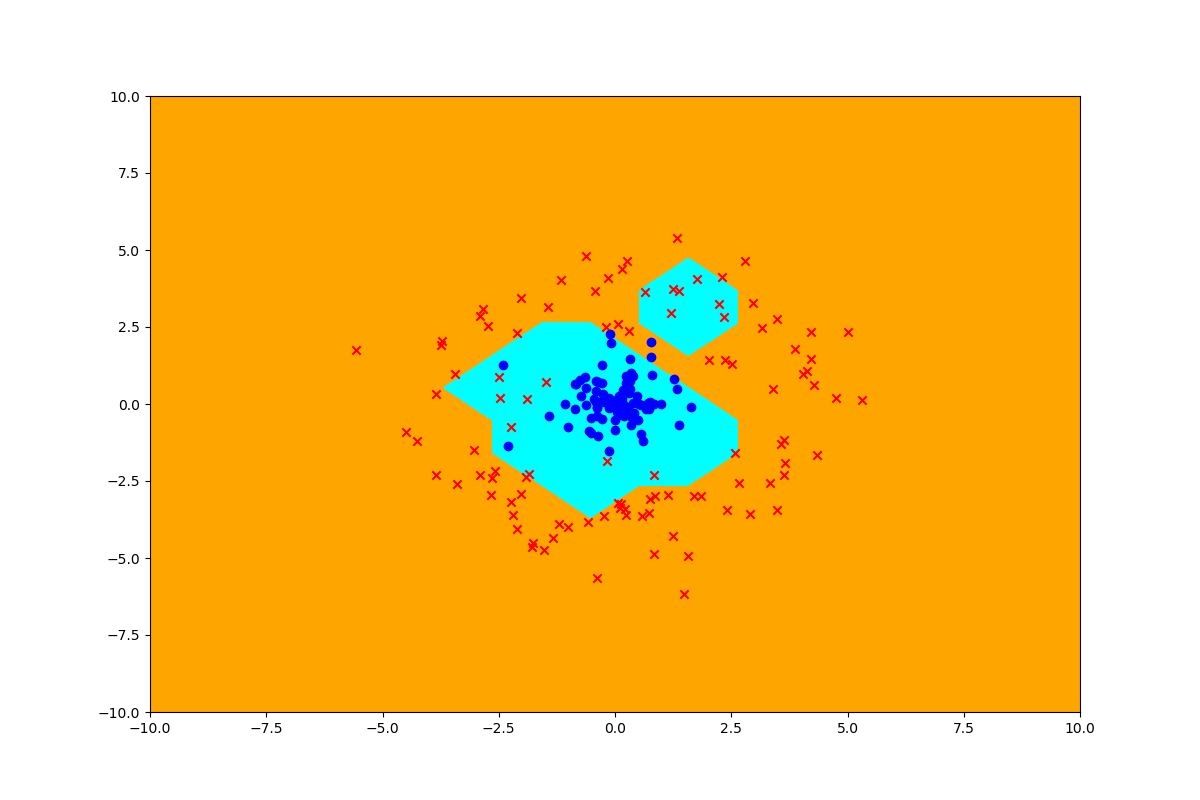
\includegraphics[width=0.65\linewidth]{03-perceptron/perceptron_rbf_output.png}
    \caption{Perceptron classifier plot for radial basis function kernel (Note: This is for reference only. You are not required to submit a plot.)}
\end{figure}

\begin{figure}[H]
	\centering
	\vspace{2mm}
	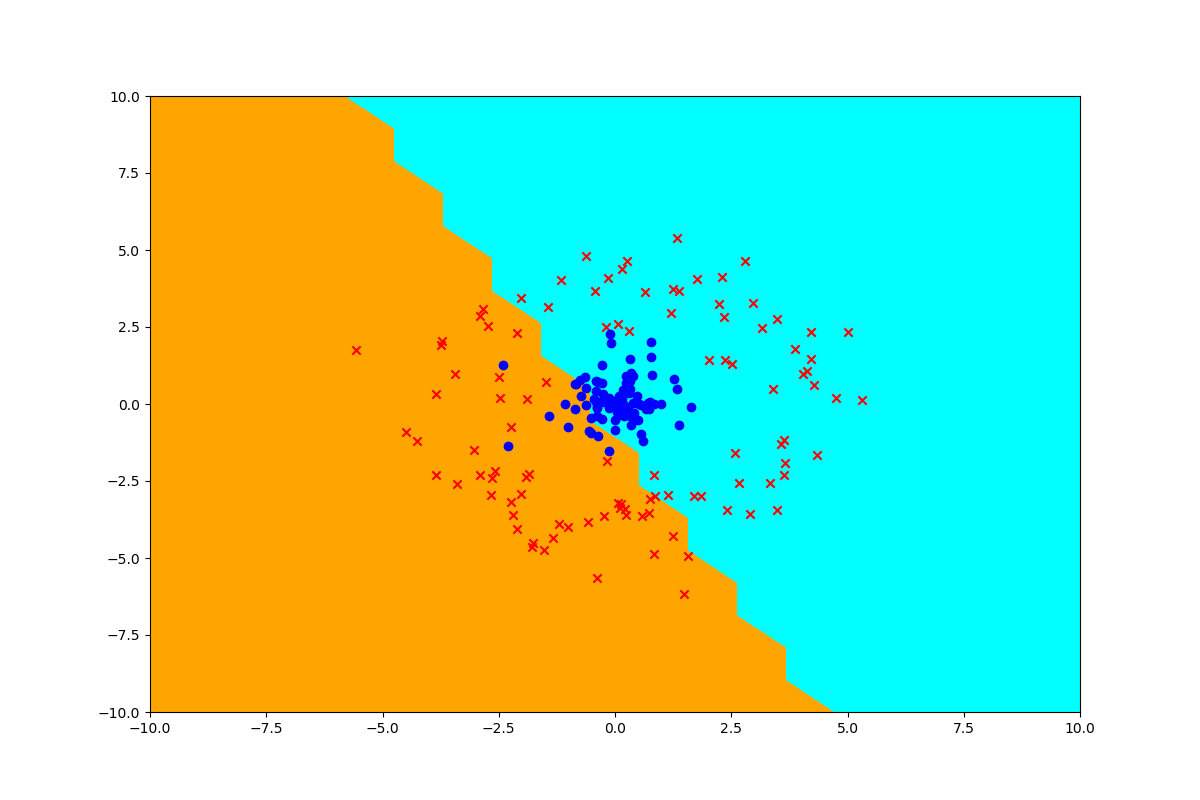
\includegraphics[width=0.65\linewidth]{03-perceptron/perceptron_dot_output.png}
    \caption{Perceptron classifier plot for dot-product kernel (Note: This is for reference only. You are not required to submit a plot.)}
\end{figure}

  \input{03-perceptron/03-failure}
\end{enumerate}
